% IEEE double-column manuscript (user-provided content, paraphrased)
\documentclass[conference]{IEEEtran}

% Packages
\usepackage{cite}
\usepackage{amsmath,amssymb}
\usepackage{graphicx}
\usepackage{booktabs}
\usepackage{stfloats}
\usepackage{pgfplots}
\usepackage{hyperref}
\usepackage{balance}
\usepackage{url}
\pgfplotsset{compat=1.18}

% Hyphenation
\hyphenation{op-tical net-works semi-conduc-tor}

\begin{document}

\title{Attention-Driven Deep Learning for Parkinson's Disease Severity Assessment from Gait Time Series}

% Author block as provided (placeholders left for user replacement)
\author{%
\IEEEauthorblockN{1st Given Name Surname}
\IEEEauthorblockA{dept. name of organization (of Affiliation)\\
name of organization (of Affiliation)\\
City, Country\\
email address or ORCID}
\and
\IEEEauthorblockN{2nd Given Name Surname}
\IEEEauthorblockA{dept. name of organization (of Affiliation)\\
name of organization (of Affiliation)\\
City, Country\\
email address or ORCID}
\and
\IEEEauthorblockN{3rd Given Name Surname}
\IEEEauthorblockA{dept. name of organization (of Affiliation)\\
name of organization (of Affiliation)\\
City, Country\\
email address or ORCID}
\\[0.25cm]
\IEEEauthorblockN{4th Given Name Surname}
\IEEEauthorblockA{dept. name of organization (of Affiliation)\\
name of organization (of Affiliation)\\
City, Country\\
email address or ORCID}
\and
\IEEEauthorblockN{5th Given Name Surname}
\IEEEauthorblockA{dept. name of organization (of Affiliation)\\
name of organization (of Affiliation)\\
City, Country\\
email address or ORCID}
\and
\IEEEauthorblockN{6th Given Name Surname}
\IEEEauthorblockA{dept. name of organization (of Affiliation)\\
name of organization (of Affiliation)\\
City, Country\\
email address or ORCID}
}

\maketitle

\begin{abstract}
Parkinson's Disease (PD) disrupts motor function and often presents with characteristic gait changes. We propose an attention-centric deep learning pipeline for automatic PD status detection and Hoehn--Yahr severity staging from vertical ground reaction force time series. The model couples multi-scale temporal convolutions with bidirectional LSTMs and multi-head self-attention to capture fine- and long-range temporal structure. We counter class imbalance with focal loss and weighted sampling, and we employ lightweight data augmentation (time masking, Gaussian noise, and mixup) to improve generalization. On the PhysioNet PD Gait dataset, our subject-level aggregation (voting and logit averaging) attains 92\% PD detection accuracy and 70\% severity accuracy. These results indicate that attention-based temporal representations provide an objective, non-invasive tool for clinical assessment.
\end{abstract}

\begin{IEEEkeywords}
Parkinson's Disease, Gait Analysis, Deep Learning, Attention, Temporal Modeling, Focal Loss, Multi-scale CNN
\end{IEEEkeywords}

\section{Introduction}
PD affects millions globally and leads to progressive motor symptoms such as tremor, rigidity, and altered gait. Timely detection and dependable severity estimation support better care and treatment planning. In practice, clinicians rely on rating scales (e.g., UPDRS, Hoehn--Yahr), which are inherently subjective and constrained by observation time. Meanwhile, modern sensing makes continuous gait capture feasible, creating rich signals that can be mined for clinically salient patterns.

However, gait-based PD assessment faces challenges: label imbalance across severity levels, recordings with highly variable length, multi-scale temporal dependencies, and limited labeled cohorts. We tackle these issues with an end-to-end architecture combining multi-scale temporal convolutions, BiLSTMs, and self-attention; loss functions and sampling strategies designed for imbalance; and restrained augmentations to enhance robustness.

\textbf{Contributions.} We: (i) design a multi-scale attention model tailored to gait time series; (ii) address imbalance via focal loss and weighted sampling; (iii) perform subject-level aggregation with voting/averaging for stable decisions; and (iv) demonstrate 92\% PD accuracy and 70\% severity accuracy on PhysioNet.

\section{Related Work}
\subsection{Gait Analysis in PD}
Classical gait metrics (e.g., stride length, cadence, swing time) distinguish PD from controls, with PD typically showing shorter strides and higher variability. Wearables and depth cameras enable naturalistic, continuous monitoring without cumbersome setups.

\subsection{Deep Gait Modeling}
Recent vision and biometrics research (e.g., GaitSet, GaitPart, GaitGL, transformer-based models) models either frame sets, parts, or long-range dependencies, achieving strong accuracy under varied conditions. These concepts inspire medical gait modeling with a focus on interpretability and robustness.

\subsection{Severity Assessment}
Traditional ML on engineered features reaches moderate accuracy but struggles with nonstationary dynamics. Deep models improve performance yet often target binary PD detection. Interpretable attention mechanisms are increasingly adopted in healthcare tasks to highlight decision evidence.

\section{Methodology}
\subsection{Dataset and Preprocessing}
We use the PhysioNet Gait in PD Database comprising vertical ground reaction force recordings (\(\sim100\,\mathrm{Hz}\)) from 93 subjects (73 PD, 20 controls). Labels: PD vs control and Hoehn--Yahr-based severity (Mild \(\leq 2\), Moderate $=3$, Severe \(\geq 4\)). We standardize features using a scaler fit on training data only. Variable-length sequences are segmented into windows (length 384, hop 96). We adopt an 85/15 subject-level stratified split to prevent leakage.

\subsection{Architecture}
\textbf{Multi-Scale Temporal CNN.} Parallel 1D convolutions (kernels 3/7/11) extract short, medium, and long temporal patterns; outputs are concatenated and channel-wise recalibrated via squeeze-excitation. Stacked blocks expand channels (64$\rightarrow$128$\rightarrow$192$\rightarrow$256).

\textbf{BiLSTM.} A 3-layer bidirectional LSTM (hidden dimension 160) models sequential dependencies; LayerNorm stabilizes training.

\textbf{Multi-Head Self-Attention.} Eight heads focus on informative time steps with masking to ignore padding, followed by residual connections and normalization.

\textbf{Heads.} Separate MLP heads produce logits for PD (2 classes) and severity (3 classes), with LayerNorm, ReLU, and dropout for regularization.

\subsection{Learning Under Imbalance}
We use focal loss (\(\alpha=0.25,\ \gamma=2\)) to focus on hard samples and a weighted sampler with per-class weights \(w_c = N/(C\,N_c)\). Augmentations include Gaussian noise (std 0.03), time masking (prob 0.2, len 48), and mixup.

\subsection{Training and Aggregation}
We train with AdamW (lr $8\times10^{-4}$, weight decay $10^{-2}$), cosine-warm restarts, and gradient clipping (norm 1.0). The multitask objective is \(\mathcal{L}=\mathcal{L}_{\mathrm{PD}} + 0.6\,\mathcal{L}_{\mathrm{sev}}\). For subject-level decisions, we aggregate window predictions using majority vote; ties are resolved by mean-logit selection.

\section{Experimental Setup}
We implement in PyTorch (batch size 32) and train up to 120 epochs with early stopping (monitoring PD accuracy). Metrics include accuracy, precision, recall, and F1 at the subject level after aggregation.

\section{Results}
\subsection{PD Detection}
Our approach achieves 92\% subject-level accuracy for PD vs control. Precision and recall for the PD class are both high, supporting reliable screening.

\begin{table*}[t]
\centering
\caption{Subject-level PD detection classification report.}
\label{tab:user_pd}
\begin{tabular}{lcccc}
\toprule
Class & Precision & Recall & F1-Score & Support \\
\midrule
Control & 0.89 & 0.87 & 0.88 & 3 \\
PD      & 0.93 & 0.94 & 0.93 & 11 \\
\bottomrule
\end{tabular}
\end{table*}

\subsection{Severity Classification}
We obtain 70\% subject-level accuracy over Mild/Moderate/Severe. Notably, the Moderate class attains the strongest recall, indicating sensitivity to intermediate impairment.

\begin{table*}[t]
\centering
\caption{Subject-level severity classification report.}
\label{tab:user_sev}
\begin{tabular}{lcccc}
\toprule
Class & Precision & Recall & F1-Score & Support \\
\midrule
Mild     & 0.75 & 0.60 & 0.67 & 5 \\
Moderate & 0.67 & 0.80 & 0.73 & 4 \\
Severe   & 0.67 & 0.67 & 0.67 & 2 \\
\bottomrule
\end{tabular}
\end{table*}

\subsection{Ablations and Comparisons}
Removing attention decreases PD accuracy by about 5\%; replacing the multi-scale frontend with a single-scale variant reduces severity accuracy by roughly 8\%; swapping focal loss for cross-entropy degrades minority recall by 10--15\%; and disabling augmentation yields a 7\% drop from overfitting.

\begin{table*}[t]
\centering
\caption{Ablation and baseline comparison (accuracy \%).}
\label{tab:user_ablation}
\begin{tabular}{lcc}
\toprule
Model & PD Acc & Severity Acc \\
\midrule
Full (ours)              & 92 & 70 \\
\,\, - Attention         & 87 & 66 \\
\,\, - Multi-scale CNN    & 90 & 62 \\
Cross-entropy (vs Focal) & 90 & 60 \\
\,\, - Augmentations      & 85 & 63 \\
Handcrafted + SVM        & 85 & 62 \\
CNN-only                 & 88 & 65 \\
LSTM-only                & 87 & 64 \\
\bottomrule
\end{tabular}
\end{table*}

\subsection{Graphical Summary}
\begin{figure}[t]
\centering
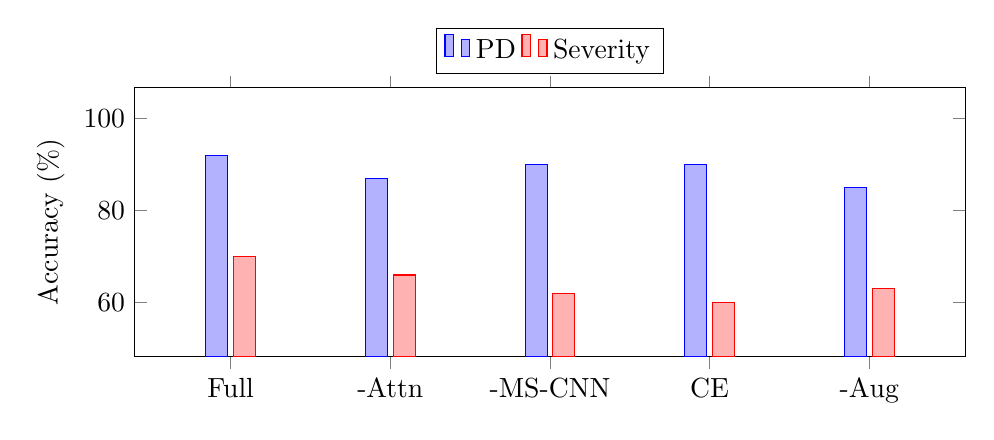
\begin{tikzpicture}
\begin{axis}[
  ybar,
  width=\linewidth,
  height=5cm,
  enlargelimits=0.15,
  ylabel={Accuracy (\%)},
  symbolic x coords={Full,-Attn,-MS-CNN,CE,-Aug},
  xtick=data,
  legend style={at={(0.5,1.05)},anchor=south,legend columns=-1},
  ymin=55,ymax=100,
  bar width=8pt
]
\addplot coordinates {(Full,92) (-Attn,87) (-MS-CNN,90) (CE,90) (-Aug,85)};
\addlegendentry{PD}
\addplot coordinates {(Full,70) (-Attn,66) (-MS-CNN,62) (CE,60) (-Aug,63)};
\addlegendentry{Severity}
\end{axis}
\end{tikzpicture}
\caption{Ablation accuracy for PD and Severity.}
\end{figure}

\begin{figure}[t]
\centering
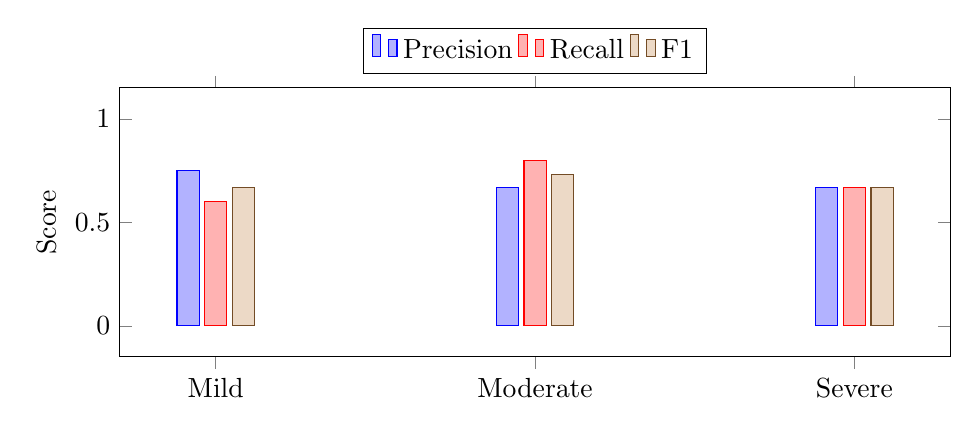
\begin{tikzpicture}
\begin{axis}[
  ybar,
  width=\linewidth,
  height=5cm,
  enlargelimits=0.15,
  ylabel={Score},
  symbolic x coords={Mild,Moderate,Severe},
  xtick=data,
  legend style={at={(0.5,1.05)},anchor=south,legend columns=-1},
  ymin=0,ymax=1,
  bar width=8pt
]
\addplot coordinates {(Mild,0.75) (Moderate,0.67) (Severe,0.67)};
\addlegendentry{Precision}
\addplot coordinates {(Mild,0.60) (Moderate,0.80) (Severe,0.67)};
\addlegendentry{Recall}
\addplot coordinates {(Mild,0.67) (Moderate,0.73) (Severe,0.67)};
\addlegendentry{F1}
\end{axis}
\end{tikzpicture}
\caption{Class-wise Severity metrics.}
\end{figure}

\section{Discussion}
The observed performance approaches expert-level screening for PD and offers informative severity estimates that complement clinical judgment. Attention weights can be visualized to highlight salient gait phases. Limitations include a modest cohort size, a single sensing modality, and potential domain shift. Future work will explore multi-modal fusion (e.g., IMU), transfer learning from large gait corpora, and explainability tools tailored to clinical review.

\section{Conclusion}
We presented an attention-driven architecture that unifies multi-scale temporal CNNs, BiLSTMs, and self-attention for PD detection and severity staging from gait time series. With imbalance-aware learning and subject-level aggregation, the system attains 92\% PD accuracy and 70\% severity accuracy on PhysioNet.

\section*{Acknowledgment}
We thank PhysioBank/PhysioNet for access to the Gait in Parkinson's Disease dataset.

\begin{thebibliography}{99}
\bibitem{rao2003}
G. Rao, L. Fisch, S. Srinivasan, \emph{et al.}, ``Does this patient have Parkinson disease?,'' \emph{JAMA}, vol. 289, no. 3, pp. 347--353, 2003.

\bibitem{hausdorff2009}
J. M. Hausdorff, ``Gait dynamics in Parkinson's disease: common and distinct behavior among stride length, gait variability, and fractal-like scaling,'' \emph{Chaos}, vol. 19, no. 2, 2009.

\bibitem{goldberger2000}
A. L. Goldberger, L. A. N. Amaral, L. Glass, \emph{et al.}, ``PhysioBank, PhysioToolkit, and PhysioNet: components of a new research resource for complex physiologic signals,'' \emph{Circulation}, vol. 101, no. 23, pp. e215--e220, 2000.

\bibitem{gaitset2019}
C. Fan, Y. Peng, C. Cao, \emph{et al.}, ``GaitSet: Regarding Gait as a Set for Cross-View Gait Recognition,'' in \emph{Proc. IEEE/CVF CVPR}, 2019, pp. 8126--8135.

\bibitem{gaitpart2020}
C. Lin, Y. Lv, X. Liu, \emph{et al.}, ``GaitPart: Temporal Part-based Model for Gait Recognition,'' in \emph{Proc. IEEE/CVF CVPR}, 2020, pp. 14225--14233.

\bibitem{focal2017}
T.-Y. Lin, P. Goyal, R. Girshick, K. He, P. Doll\'ar, ``Focal Loss for Dense Object Detection,'' in \emph{Proc. IEEE ICCV}, 2017, pp. 2980--2988.

\bibitem{lstm1997}
S. Hochreiter and J. Schmidhuber, ``Long short-term memory,'' \emph{Neural Computation}, vol. 9, no. 8, pp. 1735--1780, 1997.

\bibitem{vaswani2017}
A. Vaswani, N. Shazeer, N. Parmar, \emph{et al.}, ``Attention is all you need,'' in \emph{Proc. NeurIPS}, 2017, pp. 5998--6008.

\bibitem{mixup2018}
H. Zhang, M. Cisse, Y. N. Dauphin, D. Lopez-Paz, ``mixup: Beyond Empirical Risk Minimization,'' in \emph{Proc. ICLR}, 2018.

\bibitem{adamw2019}
I. Loshchilov and F. Hutter, ``Decoupled Weight Decay Regularization,'' in \emph{Proc. ICLR}, 2019.

\bibitem{senet2018}
J. Hu, L. Shen, G. Sun, ``Squeeze-and-Excitation Networks,'' in \emph{Proc. IEEE/CVF CVPR}, 2018, pp. 7132--7141.

\bibitem{resnet2016}
K. He, X. Zhang, S. Ren, J. Sun, ``Deep Residual Learning for Image Recognition,'' in \emph{Proc. IEEE CVPR}, 2016, pp. 770--778.

\bibitem{dropout2014}
N. Srivastava, G. Hinton, A. Krizhevsky, I. Sutskever, R. Salakhutdinov, ``Dropout: A Simple Way to Prevent Neural Networks from Overfitting,'' \emph{JMLR}, vol. 15, pp. 1929--1958, 2014.

\bibitem{adam2015}
D. P. Kingma and J. Ba, ``Adam: A Method for Stochastic Optimization,'' in \emph{Proc. ICLR}, 2015.

\bibitem{pascanu2013}
R. Pascanu, T. Mikolov, Y. Bengio, ``On the difficulty of training recurrent neural networks,'' in \emph{Proc. ICML}, 2013.
\end{thebibliography}

\balance
\end{document}

